%%%%%%%%%%%%%%%%%%%%%%%%%%%%%%%%%%%%%%%%%
% Beamer Presentation
% LaTeX Template
% Version 1.0 (10/11/12)
%
% This template has been downloaded from:
% http://www.LaTeXTemplates.com
%
% License:
% CC BY-NC-SA 3.0 (http://creativecommons.org/licenses/by-nc-sa/3.0/)
%
%%%%%%%%%%%%%%%%%%%%%%%%%%%%%%%%%%%%%%%%%

%----------------------------------------------------------------------------------------
%	PACKAGES AND THEMES
%----------------------------------------------------------------------------------------

\documentclass{beamer}

\mode<presentation> {

% The Beamer class comes with a number of default slide themes
% which change the colors and layouts of slides. Below this is a list
% of all the themes, uncomment each in turn to see what they look like.

%\usetheme{default}
%\usetheme{AnnArbor}
%\usetheme{Antibes}
%\usetheme{Bergen}
%\usetheme{Berkeley}
%\usetheme{Berlin}
%\usetheme{Boadilla}
%\usetheme{CambridgeUS}
%\usetheme{Copenhagen}
%\usetheme{Darmstadt}
%\usetheme{Dresden}
%\usetheme{Frankfurt}
%\usetheme{Goettingen}
%\usetheme{Hannover}
%\usetheme{Ilmenau}
%\usetheme{JuanLesPins}
%\usetheme{Luebeck}
\usetheme{Madrid}
%\usetheme{Malmoe}
%\usetheme{Marburg}
%\usetheme{Montpellier}
%\usetheme{PaloAlto}
%\usetheme{Pittsburgh}
%\usetheme{Rochester}
%\usetheme{Singapore}
%\usetheme{Szeged}
%\usetheme{Warsaw}

% As well as themes, the Beamer class has a number of color themes
% for any slide theme. Uncomment each of these in turn to see how it
% changes the colors of your current slide theme.

%\usecolortheme{albatross}
%\usecolortheme{beaver}
%\usecolortheme{beetle}
%\usecolortheme{crane}
%\usecolortheme{dolphin}
%\usecolortheme{dove}
%\usecolortheme{fly}
%\usecolortheme{lily}
%\usecolortheme{orchid}
%\usecolortheme{rose}
%\usecolortheme{seagull}
%\usecolortheme{seahorse}
%\usecolortheme{whale}
%\usecolortheme{wolverine}

%\setbeamertemplate{footline} % To remove the footer line in all slides uncomment this line
%\setbeamertemplate{footline}[page number] % To replace the footer line in all slides with a simple slide count uncomment this line

%\setbeamertemplate{navigation symbols}{} % To remove the navigation symbols from the bottom of all slides uncomment this line
}

\usepackage{graphicx} % Allows including images
\usepackage{booktabs} % Allows the use of \toprule, \midrule and \bottomrule in tables

%----------------------------------------------------------------------------------------
%	TITLE PAGE
%----------------------------------------------------------------------------------------

\title[Spread of Forest Fire]{The influence of different variables on the spread of Forest Fire} % The short title appears at the bottom of every slide, the full title is only on the title page

\author{Tom Peerdeman \& Ren\'e Aparicio Saez} % Your name

\date{\today} % Date, can be changed to a custom date

\begin{document}

\begin{frame}
\titlepage % Print the title page as the first slide
\end{frame}

\begin{frame}
\frametitle{Overview} % Table of contents slide, comment this block out to remove it
\tableofcontents % Throughout your presentation, if you choose to use \section{} and \subsection{} commands, these will automatically be printed on this slide as an overview of your presentation
\end{frame}

%----------------------------------------------------------------------------------------
%	PRESENTATION SLIDES
%----------------------------------------------------------------------------------------

%------------------------------------------------
\section{Intro Forest Fire} 
%------------------------------------------------

\begin{frame}
\frametitle{Introduction}
\begin{itemize}
\item{Cellular Automata}
\item{Different Grids}
\item{Probabilities instead of set rules}
\end{itemize}
\end{frame}

%------------------------------------------------
\section{Different Grids and their Neighborhoods} 
%------------------------------------------------

\begin{frame}
\frametitle{Cartesian \& hexagonal Grids}
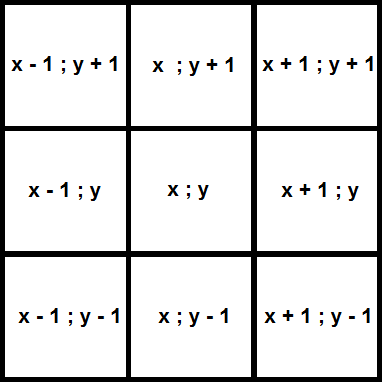
\includegraphics[width=0.5\textwidth]{imgs/cartesian.png}
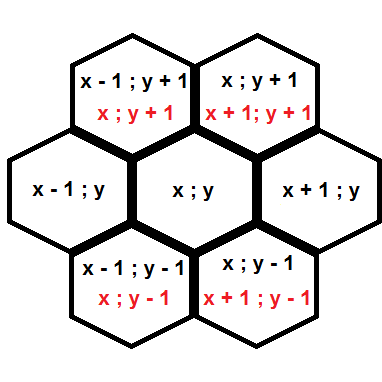
\includegraphics[width=0.5\textwidth]{imgs/hexagonal.png}
\end{frame}

\begin{frame}
\frametitle{Triangular Grids}
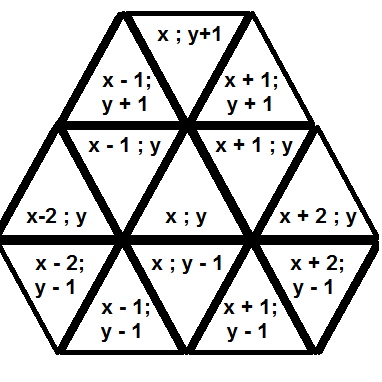
\includegraphics[width=0.5\textwidth]{imgs/triangle1.png}
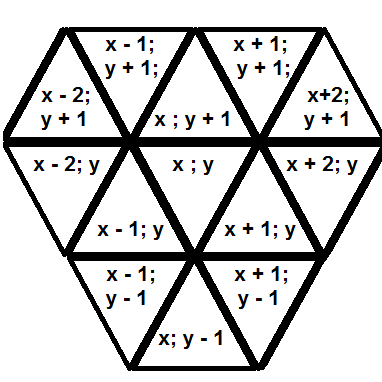
\includegraphics[width=0.5\textwidth]{imgs/triangle2.png}
\end{frame}

\begin{frame}
\frametitle{Extended Cartesian \& hexagonal Grid}
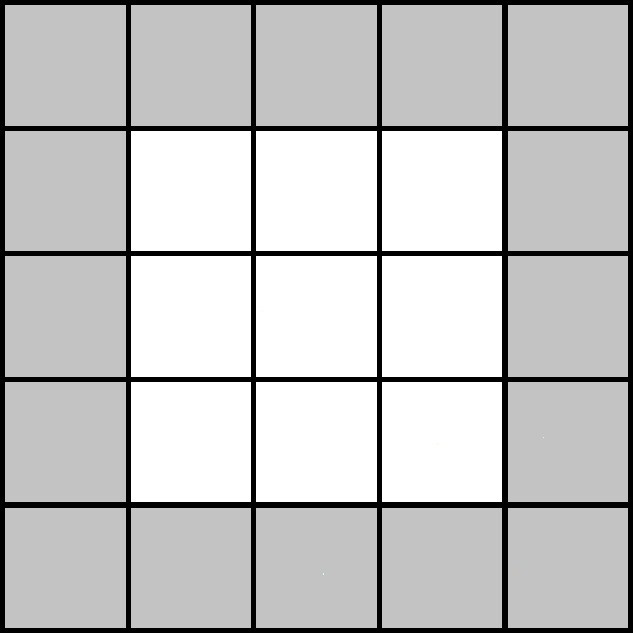
\includegraphics[width=0.5\textwidth]{imgs/extendedcartesian.png}
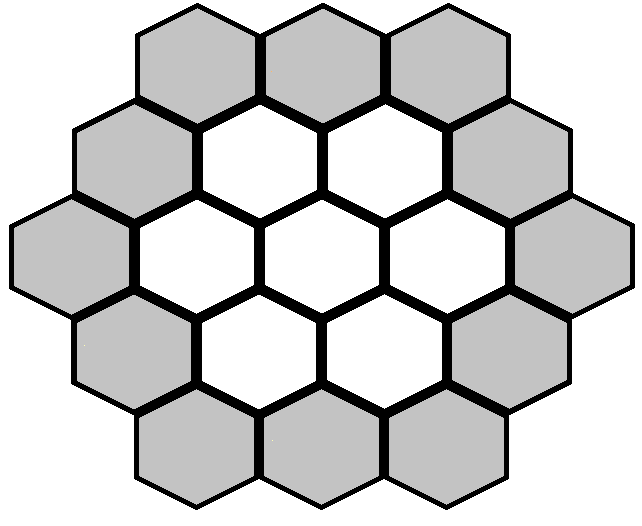
\includegraphics[width=0.5\textwidth]{imgs/extendedhexagonal.png}
\end{frame}

\begin{frame}
\frametitle{Extended Triangular Grids}
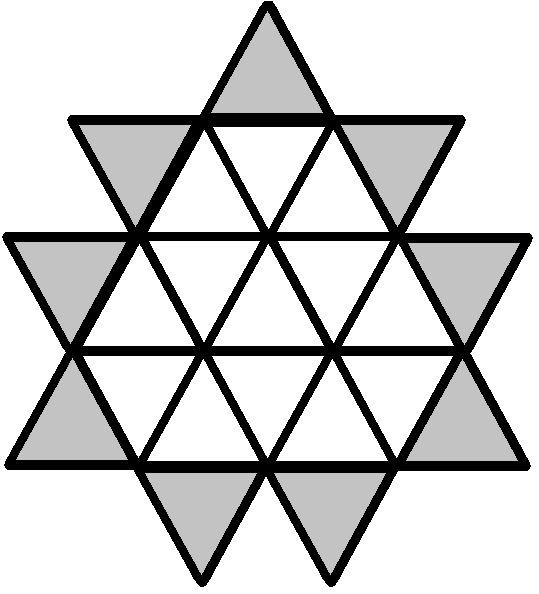
\includegraphics[width=0.5\textwidth]{imgs/extendedtriangle1.png}
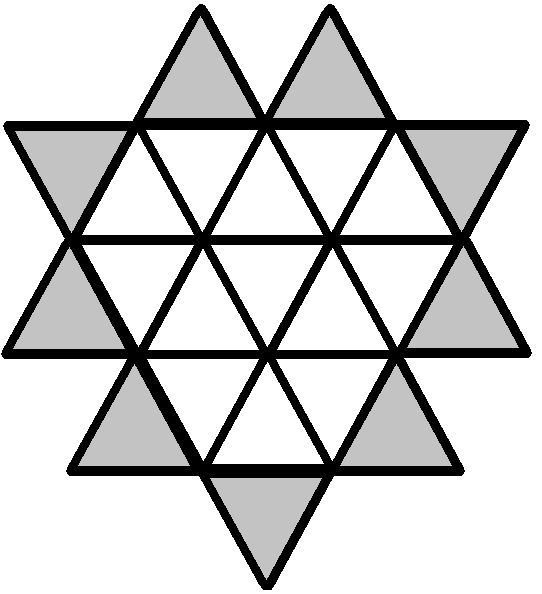
\includegraphics[width=0.5\textwidth]{imgs/extendedtriangle2.png}
\end{frame}

%------------------------------------------------
\section{Simulation probabilities} 
%------------------------------------------------

\begin{frame}
\frametitle{Simulation probabilities}
\begin{itemize}
\item{Spread Probability}
\item{Extinguish Probability}
\end{itemize}
\end{frame}

%------------------------------------------------
\section{Experiments and interpretation} 
%------------------------------------------------

\begin{frame}
\frametitle{Normal neighborhoods}
No water or roads, no firefighting, no extended neighborhood
\centering
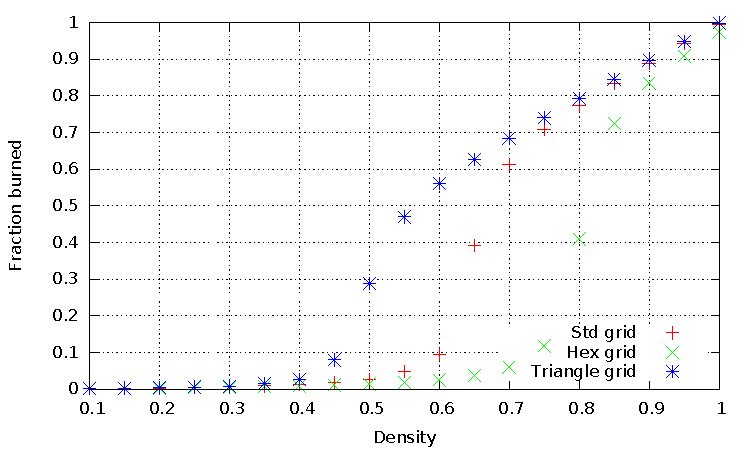
\includegraphics[width=\textwidth]{imgs/plot/ex1/fracburned.pdf}
\end{frame}

\begin{frame}
\frametitle{Normal neighborhoods}
water and roads, no firefighting, no extended neighborhood
\centering
\includegraphics[width=\textwidth]{imgs/plot/ex3/fracburned.pdf}
\end{frame}

\begin{frame}
\frametitle{Normal neighborhoods}
water and roads, firefighting, no extended neighborhood
\centering
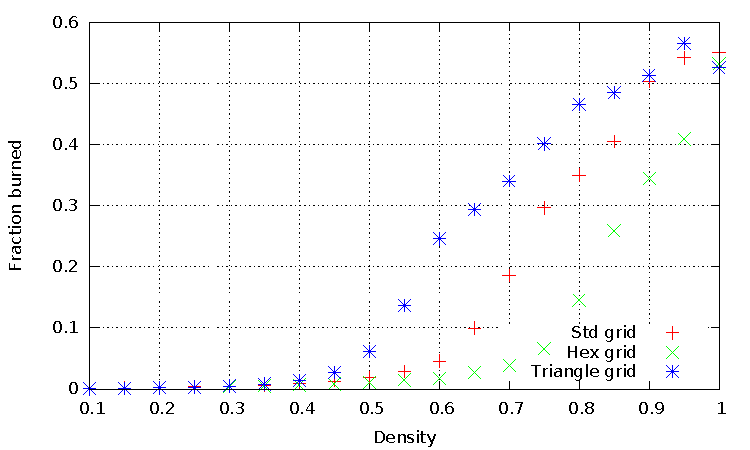
\includegraphics[width=\textwidth]{imgs/plot/ex5/fracburned.pdf}
\end{frame}

\begin{frame}
\frametitle{Extended neighborhoods}
No water or roads, no firefighting, extended neighborhood
\centering
\includegraphics[width=\textwidth]{imgs/plot/ex2/fracburned.pdf}
\end{frame}

\begin{frame}
\frametitle{Extended neighborhoods}
water and roads, no firefighting, extended neighborhood
\centering
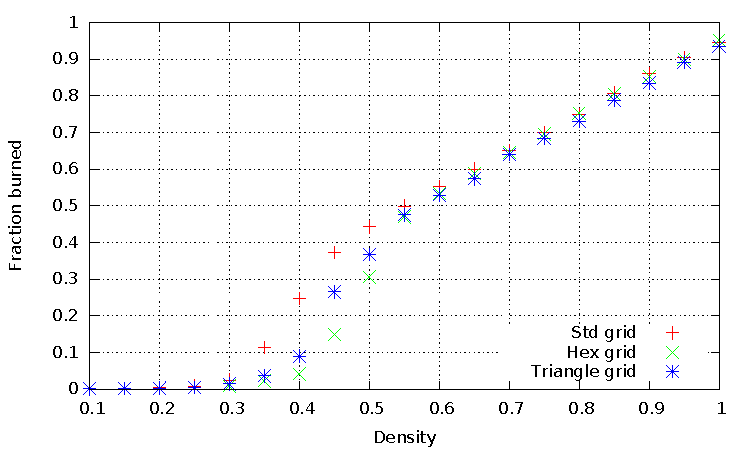
\includegraphics[width=\textwidth]{imgs/plot/ex4/fracburned.pdf}
\end{frame}

\begin{frame}
\frametitle{Extended neighborhoods}
water and roads, firefighting, extended neighborhood
\centering
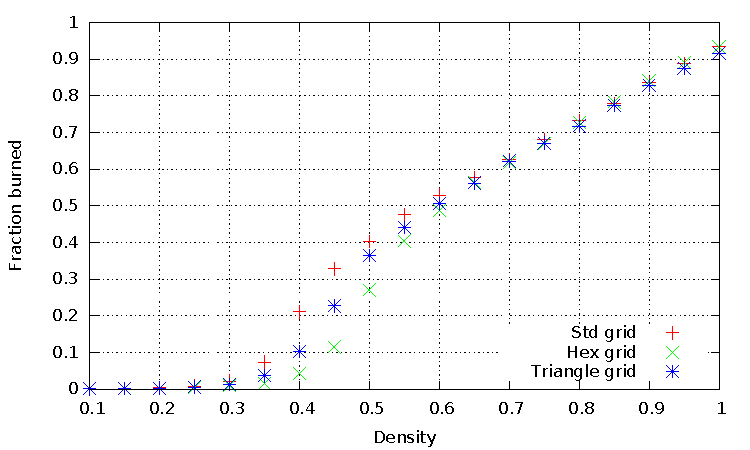
\includegraphics[width=\textwidth]{imgs/plot/ex6/fracburned.pdf}
\end{frame}
%------------------------------------------------
\section{Conclusion} 
%------------------------------------------------

\begin{frame}
\frametitle{Conclusion}
\begin{itemize}
\item{Water and roads}
\pause 
\begin{itemize}
\item[$\rightarrow$] Slows down firespread significantly
\end{itemize}
\pause 
\item{Extended Neighborhoods}
\pause 
\begin{itemize}
\item[$\rightarrow$]  Speeds up firespread
\end{itemize}
\pause
\item{Firefighting}
\pause 
\begin{itemize}
\item[$\rightarrow$]  Doesnt slow down fire
\end{itemize}
\end{itemize}
\end{frame}


%------------------------------------------------

\begin{frame}
\frametitle{References}
\footnotesize{
\begin{thebibliography}{99} % Beamer does not support BibTeX so references must be inserted manually as below
\bibitem[Smith, 2012]{p1} John Smith (2012)
\newblock Title of the publication
\newblock \emph{Journal Name} 12(3), 45 -- 678.
\end{thebibliography}
}
\end{frame}

%------------------------------------------------

\begin{frame}
\Huge{\centerline{The End}}
\end{frame}

%----------------------------------------------------------------------------------------

\end{document}